%!TEX root = thesis.tex

\chapter{Results and Evaluation}
\label{chapter:Results and Evaluation}

This chapter will cover the subsystems and steps taken that were needed to achieve the testing environment described in Chapter~\ref{chapter:Proposed architecture}. This chapter will first discuss the arrangements related to the hardware of the framework and then software related arrangements will be presented and described. After presenting the built framework, achieved results will be discussed and finally the test environment presented in this Thesis will be evaluated.

\section{Hardware arrangements}
\label{section:Hardware arrangements}

\subsection{The Robot}
\label{subsection:Robot}

\begin{figure}[ht]
  \begin{center}
    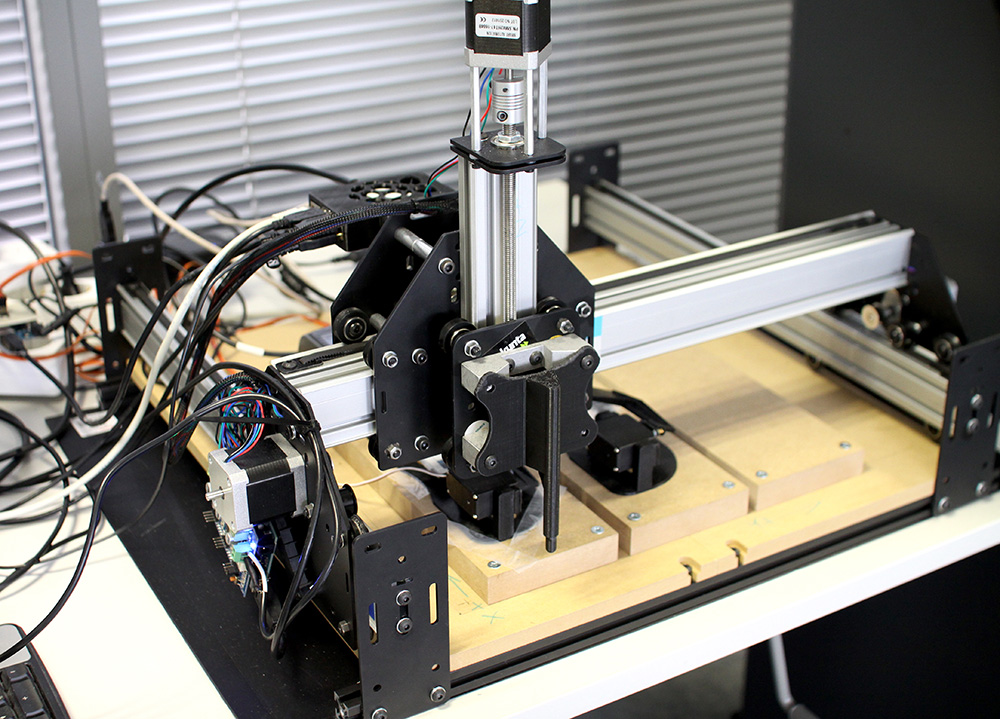
\includegraphics[width=10cm]{images/robot.jpg}
    \caption{Robot in its production state.}
    \label{fig:invalid_pin_test}
  \end{center}
\end{figure}
\FloatBarrier

\begin{figure}[ht]
  \begin{center}
    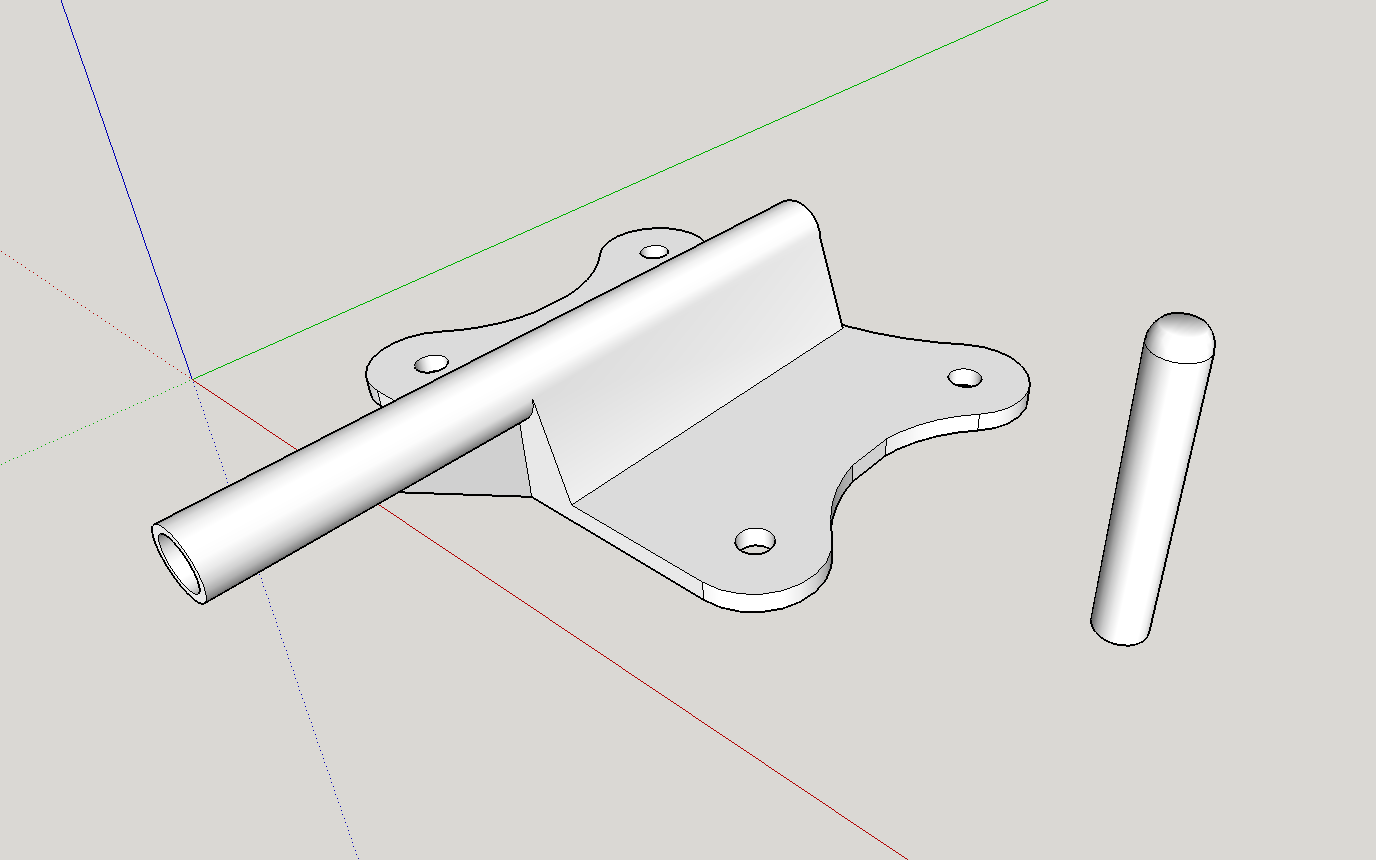
\includegraphics[width=12cm]{images/pushing_tool.png}
    \caption{CAD design of the pushing tool.}
    \label{fig:pushing_tool}
  \end{center}
\end{figure}
\FloatBarrier

\subsection{Camera arrangements}
\label{subsection:Camera Arrangements}

\begin{figure}[ht]
  \begin{center}
    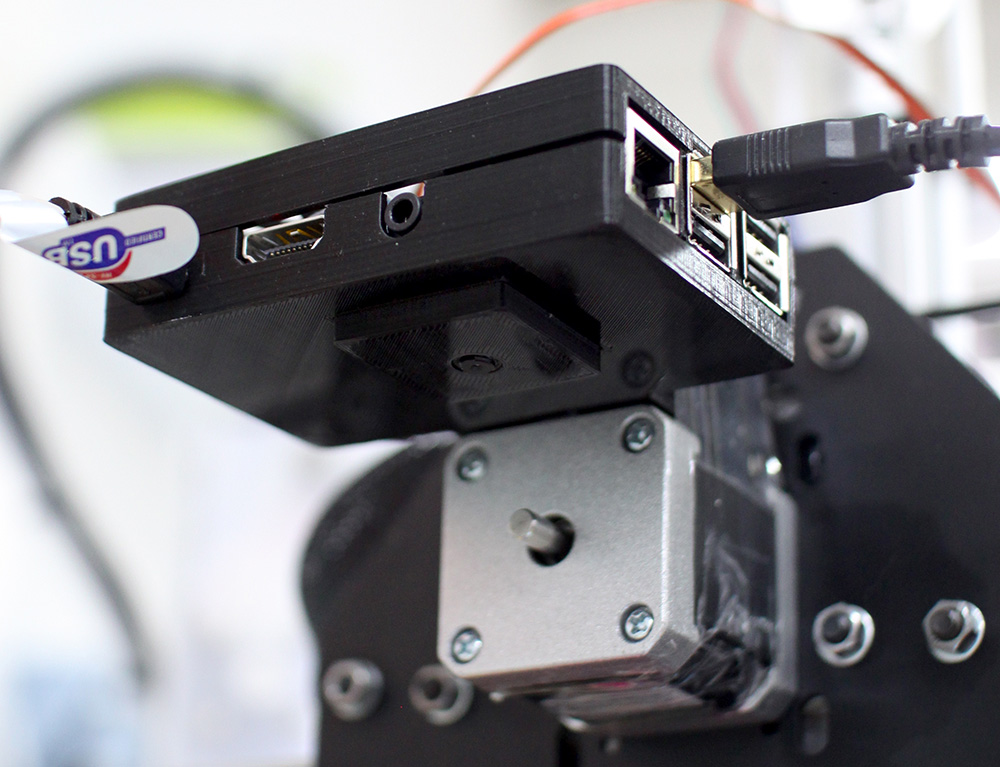
\includegraphics[width=10cm]{images/camera.jpg}
    \caption{Camera is attached to the bottom of the Raspberry Pi's enclosure.}
    \label{fig:invalid_pin_test}
  \end{center}
\end{figure}
\FloatBarrier

\subsection{Computing hardware}
\label{subsection:Computing hardware}

\subsection{Card feeder arrangements}
\label{subsection:Card feeder arrangements}

\begin{figure}[ht]
  \begin{center}
    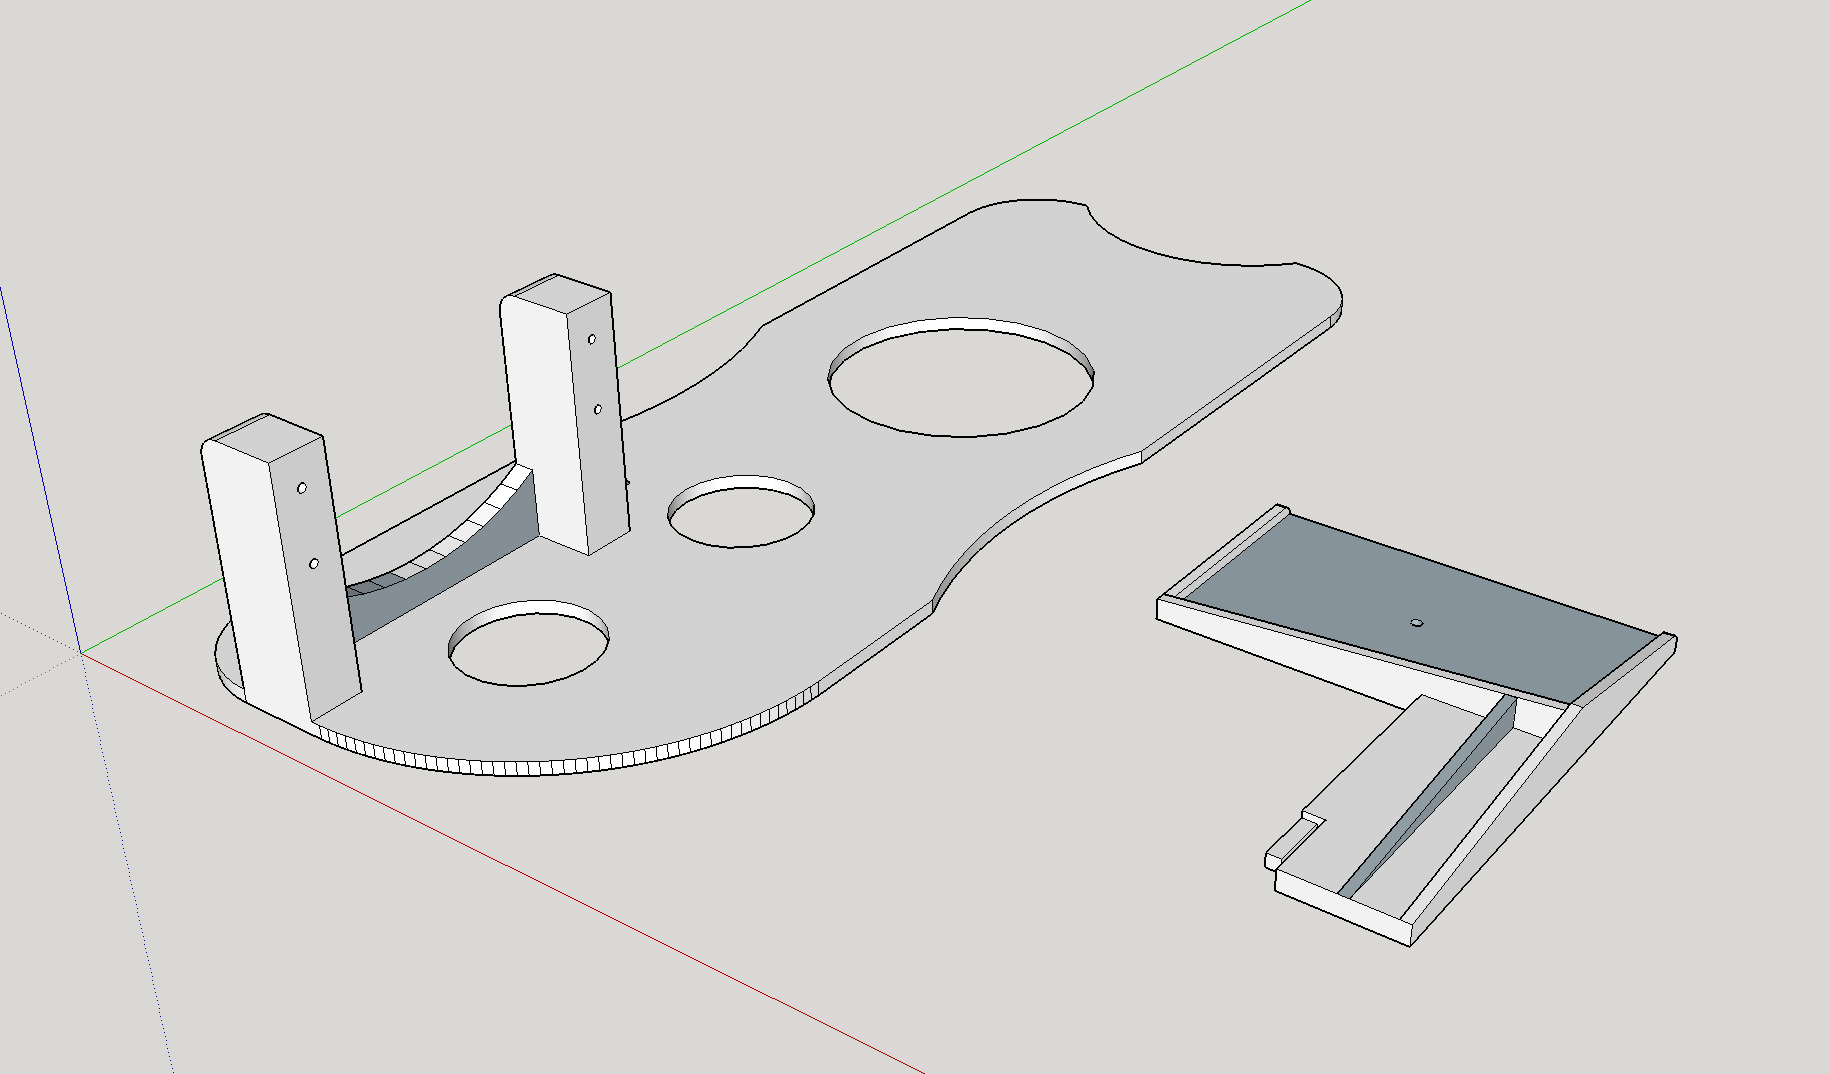
\includegraphics[width=12cm]{images/card_feeder.png}
    \caption{CAD design of the card feeder.}
    \label{fig:pushing_tool}
  \end{center}
\end{figure}
\FloatBarrier

\section{Software arrangements}
\label{section:Software arrangements}

\subsection{Software architecture}
\label{subsection:Software architecture}

\subsection{Robot Framework and libraries}
\label{subsection:Robot Framework and libraries}

\subsection{Computer vision arrangements}
\label{subsection:Computer vision arrangements}

\subsection{Test syntax}
\label{subsection:Test syntax}


\section{Results}
\label{section:Results}

\section{Evaluation}
\label{section:Evaluation}